\documentclass[../analytical_approach.tex]{subfiles}
\begin{document}
\subsubsection{Joint Positions}
\label{sec:jointpositions}
\iffalse
    \begin{figure}[H]
        \centering
        \caption{Joint Portfolio}
        \label{fig:jointpi}
        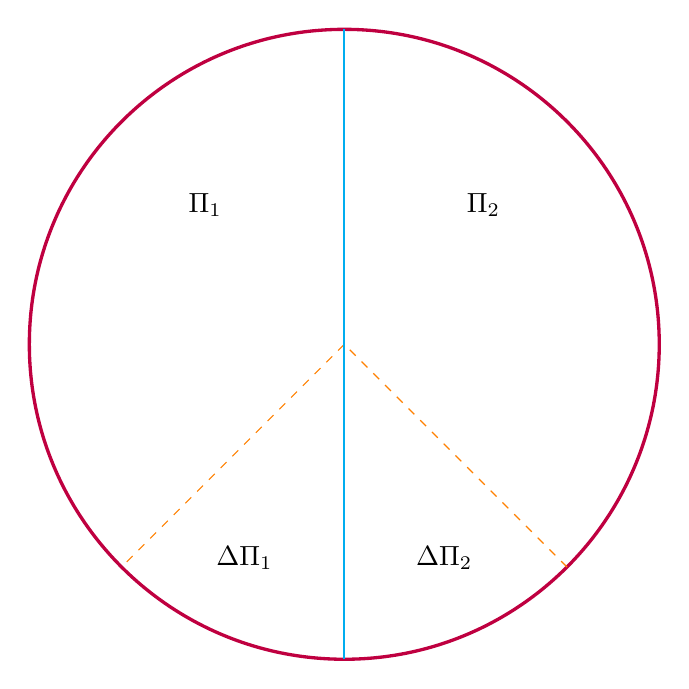
\begin{tikzpicture}
            \draw[very thick,purple] (0,0) circle [radius=4] ;
            \draw[dashed,orange] (315:4) -- (0,0) -- (225:4);
            \draw[thick,cyan] (90:4) -- (0,0) -- (270:4);
            \node at (135:2.5) {$\Pi_1$};
            \node at (45:2.5) {$\Pi_2$};
            \node at (245:3) {$\Delta\Pi_1$};
            \node at (295:3) {$\Delta\Pi_2$};
        \end{tikzpicture}
    \end{figure}
\fi
We have just discussed how to estimate the VaR a portfolio containing a single stock.
Now we consider the VaR estimate of a joint portfolio which is worth:  $\Pi = (\Pi_1+\Pi_2)$.
Our VaR estimate of this portfolio is not simply the combination of VaR for $\Pi_1$ and VaR for $\Pi_2$.
This is because losses in $\Pi_1$ do not necessarily coincide with losses in $\Pi_2$.\\
Likewise, the change in the value of our portfolio is worth:
\begin{equation}
    \label{eqn:deltajointpi}
    \Delta\Pi=\bigg(\Delta\Pi_1\sim\phi\big(0,\Pi^2_1\sigma^2_1\Delta t\big) + \Delta\Pi_2\sim\phi\big(0,\Pi^2_2\sigma^2_2\Delta t\big)\bigg)
\end{equation}
We know the distributions of both parts of the portfolio.
What about the sum of the distributions?
Firstly, expectation of a sum is equal to the sum of expectations and both parts of $\Delta\Pi$ have a mean of zero due to the simplification we made in equation~\ref{eqn:stochastic2}.
So:
\begin{equation}
    \label{eqn:sumexpectations}
    \mathbb{E}\Delta\Pi=\mathbb{E}(\Delta\Pi_1 + \Delta\Pi_2) = \mathbb{E}\Delta\Pi_1 + \mathbb{E}\Delta\Pi_2 = 0
\end{equation}
Secondly, any linear combination of Gaussian variables s is Gaussian and both parts of $\Delta\Pi$ are Gaussian.
As such, what remains is to find the variance of $\Delta\Pi_1 + \Delta\Pi_2$.

The variance of $\Delta\Pi_1$ is defined as $\text{var}(\Delta\Pi_1)=\mathbb{E}(\Delta\Pi_1-\mathbb{E}\Delta\Pi_1)^2$.
The variance of $(\Delta\Pi_1+\Delta\Pi_2)$ is:
\begin{multline}
    \label{eqn:jointvar}
    \text{var}(\Delta\Pi_1+\Delta\Pi_2) =\\ \mathbb{E}\big[(\Delta\Pi_1+\Delta\Pi_2)-\mathbb{E}(\Delta\Pi_1+\Delta\Pi_2)\big]^2
    %\\= \mathbb{E}\big[\Delta\Pi_1+\Delta\Pi_2-\mathbb{E}\Delta\Pi_1-\mathbb{E}\Delta\Pi_2)\big]^2 =  \mathbb{E}\big[(\Delta\Pi_1-\mathbb{E}\Delta\Pi_1)+(\Delta\Pi_2-\mathbb{E}\Delta\Pi_2)\big]^2 
    %\\= \mathbb{E}\big[(\Delta\Pi_1-\mathbb{E}\Delta\Pi_1)^2+(\Delta\Pi_2-\mathbb{E}\Delta\Pi_2)^2+2(\Delta\Pi_1-\mathbb{E}\Delta\Pi_1)(\Delta\Pi_2-\mathbb{E}\Delta\Pi_2)\big]^2 
    \\= \underbrace{\mathbb{E}(\Delta\Pi_1-\mathbb{E}\Delta\Pi_1)^2}_\textrm{variance} + \underbrace{\mathbb{E}(\Delta\Pi_2-\mathbb{E}\Delta\Pi_2)^2}_\textrm{variance} + 2\underbrace{\mathbb{E}(\Delta\Pi_1-\mathbb{E}\Delta\Pi_1)\mathbb{E}(\Delta\Pi_2-\mathbb{E}\Delta\Pi_2)}_\textrm{covariance}
\end{multline}
As before, means are zero so:
\begin{equation}
    \label{eqn:jointvar2}
    \underbrace{\mathbb{E}(\Delta\Pi_1)^2}_\textrm{variance} + \underbrace{\mathbb{E}(\Delta\Pi_2)^2}_\textrm{variance} + 2\underbrace{\mathbb{E}(\Delta\Pi_1)\mathbb{E}(\Delta\Pi_2)}_\textrm{covariance}
\end{equation}
Since $\text{std}(\Delta\Pi_1)=\sqrt{\text{var}(\Delta\Pi_1)}$ and $\text{std}(\Delta\Pi_2)=\sqrt{\text{var}(\Delta\Pi_2})$, we can rewrite equation~\ref{eqn:jointvar2} in terms of standard deviations (i.e. volatilities), such that:
\begin{equation}
    \label{eqn:jointstdev}
    \text{std}(\Delta\Pi_1+\Delta\Pi_2) = \sqrt{\text{std}(\Delta\Pi_1)^2 + \text{std}(\Delta\Pi_2)^2 +2\rho\cdot\text{std}(\Delta\Pi_1)\cdot\text{std}(\Delta\Pi_2)}
\end{equation}
where $\rho$ is the correlation coefficient defined as:
\begin{equation}
    \label{eqn:correlation}
    \rho = \frac{\text{cov}(\Delta\Pi_1,\Delta\Pi_2)}{\text{std}(\Delta\Pi_1)\cdot\text{std}(\Delta\Pi_2)}
\end{equation}
and $-1\leq\rho\leq1$
\paragraph{Correlation\\}
\begin{figure}[H]
    \centering
    \caption{Correlation Coefficient}
    \label{fig:correlationcoefficient}
    \begin{tikzpicture}
        \begin{groupplot}[
                group style={
                        group name = the correlation coefficient
                        ,	group size = 3 by 1
                    }
                ,	footnotesize,
                ,	width=5cm
                ,	height=5cm
                ,	xmin = -0.2
                ,	xmax = 1.2
                ,	ymin = -0.2
                ,	ymax = 1.2
                ,	ytick = \empty
                ,	xtick = \empty
                ,	enlarge x limits=false
            ]
            \nextgroupplot[title={$\rho=1$}]
            \addplot[->, thick, cyan] coordinates {
                    (0.5,0.5)(1,1)
                };
            \node at (125,125) {x};
            \addplot[->,thick,purple] coordinates {
                    (0.5,0.5)(0.75,0.75)
                };
            \node at (100,80) {y};
            \nextgroupplot[title={$\rho=0$}]
            \addplot[->, thick, cyan] coordinates {
                    (0.5,0.5)(1,1)
                };
            \node at (125,125) {x};
            \addplot[->,thick,purple] coordinates {
                    (0.5,0.5)(0.25,0.75)
                };
            \node at (35,100) {y};
            \nextgroupplot[title={$\rho=-1$}]
            \addplot[->, thick, cyan] coordinates {
                    (0.5,0.5)(1,1)
                };
            \node at (125,125) {x};
            \addplot[->,thick,purple] coordinates {
                    (0.5,0.5)(0.0,0.0)
                };
            \node at (15,15) {y};
        \end{groupplot}
    \end{tikzpicture}
\end{figure}
In figure~\ref{fig:correlationcoefficient}, we illustrate the correlation of two random variable $X$ and $Y$.
As the correlation coefficient moves through $\rho = 1, \rho = 0, \rho = - 1$, we see examples of full positive correlation, independence and full negative correlation between $X$ and $Y$ respectively.
The blue length is $\text{std}(X)$ and the purple length is $\text{std}({Y})$.
We can see that $\rho$ is analogous to the cosine of the angle between the two lengths and the covariance is the scalar product.

When $X$ and $Y$ have positive correlation $\rho > 0$, they have dependency such that when $X$ is large, $Y$ will be large too.
On the other hand, when $\rho < 0$, the random variables have dependency between them but if $X$ is large $Y$ will be small.

\paragraph{Calculating VaR\\}

In calculating the standard deviation of $\Delta\Pi_1$ and $\Delta\Pi_2$, we can now find the one day VaR.
Suppose we have a confidence level $c = 99\%$, from which follows the percentile $x_{1\%}$, and a time horizon $\Delta t = N$.
We calculate our Value at Risk as
\begin{equation}
    \label{eqn:jointvar}
    V= x_{1\%}\text{std}(\Delta\Pi_1+\Delta\Pi_2)\sqrt{N}
\end{equation}
Though it may look different but this last step is, in essence, identical to equation~\ref{eqn:varsinglestock} where we find the VaR of a single stock portfolio by multiplying the standard deviation of the daily changes in portfolio $\Pi\sigma$  by $x_{1\%}\sqrt{\Delta t}$.
\end{document}